\documentclass[11pt]{article}
\usepackage[margin=1.1in]{geometry}
\usepackage{amsmath,amssymb,amsthm}
\usepackage{hyperref}
\usepackage{booktabs}
\usepackage{array}
\usepackage[protrusion=true,expansion=false]{microtype}
\usepackage{xcolor}
\usepackage{enumitem}
\usepackage{titlesec}
\usepackage{tikz}
\usepackage{float}
\usepackage[normalem]{ulem}
\usetikzlibrary{arrows.meta,positioning,fit,shapes.geometric,calc}
\usepackage{listings}

\hypersetup{colorlinks=true, linkcolor=blue!60!black, urlcolor=blue!60!black, citecolor=blue!60!black}

\titleformat{\section}{\large\bfseries}{\thesection.}{0.7em}{}
\titleformat{\subsection}{\normalsize\bfseries}{\thesubsection.}{0.6em}{}

\newcommand{\transcript}{\bigl(A_{1},A_{2},\textrm{PoKs},\textrm{ctxt},T,\sigma'_{A,P},R_{\cdot\cdot},s_{1},s_{2},e_{1},e_{2}\bigr)}

% macros for the dispute-graph section
\newcommand{\op}[1]{\texttt{OP\_#1}}
\newcommand{\push}[1]{\ensuremath{\langle #1\rangle}}
\newcommand{\U}{\mathsf{U}}
\newcommand{\Hb}{\mathsf{H}}
\newcommand{\tsd}{\Delta}
\newcommand{\dl}{\delta}
\newcommand{\dlp}{\delta'}
\lstdefinestyle{script}{
  basicstyle=\ttfamily\small,
  columns=fullflexible,
  keepspaces=true,
  breaklines=true,
  frame=single,
  framerule=0.3pt,
  xleftmargin=1em,
  escapeinside={(*}{*)},
}

\newtheorem{theorem}{Theorem}
\newtheorem{definition}{Definition}
\newtheorem{remark}{Remark}
\newtheorem{lemma}{Lemma}
\newtheorem{observation}{Observation}
\usepackage[skip=0.6\baselineskip, indent=0pt]{parskip}
\title{\textbf{LN-GAP}\\Lightning governed by arbitrary programs}
\author{waxwing}

\date{September 2026 \\ \medskip Version 1.0 (draft)}

\begin{document}
\maketitle

\tableofcontents

\section{Abstract}

We propose, without any consensus change to Bitcoin, offchain bilateral contracts in Bitcoin that depend on arbitrary computation, calling this general paradigm LN-GAP (Lightning Network governed by arbitrary programs). That general idea is not new but we describe here a distinct mechanism to achieve O(1)-transactions to resolve disputed contracts onchain (that is, there is no onchain bisection), based on the use of a proof of publication ledger governed by a threshold of validators. The onchain dispute resolution depends on a threshold attestation of the validators to absence of a published entry in the ledger, and a 1 of $n$ positive signature over the entry in a novel way (we call this an elliptic curve one time signature, or EC-OTS), and in so doing allows the application of the ForceMove paradigm for the offchain game with an independent timeout clock that does not rely on facts about the Bitcoin chain itself (thus not requiring Bitcoin SPV proofs). The advantages of this construction are: publishing of entries in the ledger require only 1 of $n$ liveness, contracts are fully denominated in bitcoin and trustless modulo corruption of the (presumed large and heterogenous) majority of the PoP ledger validators, who themselves are not required to know anything about the bilateral contract details, and fraudulent equivocation is provable. Those validators are motivated by both positive fees (paid, in bitcoin, atomically with publication in LN channels) and negatively by bonds (timelocked funds that will not be compensated with fees when fraud is attributed, and burnt to miners).

\section{Introduction}

Start from the \textbf{known good} - that Lightning as a payments technology works, and works well. It aids privacy and scalability, if not perfectly addressing both, it addresses them to a large extent, at the cost of extra infrastructure for users and service providers. Once that infrastructure is in place, the \emph{payments} UI/workflow for users is as smooth as it should be\footnote{For those readers who balk at this characterization, note that the author has been paying his utility bills for years, and along with thousands of other payments during that time with near zero payment failures, on self-custodial Lightning, and for practical, not ideological, reasons, far prefers using LN as a payment technology over any existing fiat rail.}.

What's missing? Lightning already provides private, fast and cheap payments. In vague terms, I would argue that all it really misses is ``programmatic extensibility''. Take as an example this goal:

\begin{quote}
The customer wants to pay a storage service provider once per day, in sats, but wants the service provider to prove that they are upholding their agreement (with a response to a challenge for an inclusion proof), and if they fail to do so after a time window, their deposit can be taken.
\end{quote}

This is basically ``\underline{Filecoin without an altcoin}'', as realized in the system described in this paper.

\subsection{The problem of 2-party games on Lightning}

Suppose you want to play a game on Lightning, like chess, for a monetary reward, but don't want to have to trust anyone; the money should move specifically according to the agreed game rules.

I mention chess not because it's a good game to bet on (it isn't!) but because it's a game that's sufficiently complex that expressing it in onchain transactions (most specifically, proving a that move is illegal; proving that a move is legal would be way worse!) gets very expensive and we want to avoid it.

One approach to doing this offchain is called ForceMoveLINK. The idea is relatively simple: behave optimistically, and fallback to onchain transactions as the arbiter if your opponent does not follow the rules you agreed to. The reason for its name is that, once on-chain, the opponent is \emph{forced to move} by having a timeout expressed in the blockchain's consensus logic. So in Bitcoin this would mean that the Script controlling the funds has a shape like: 

\[
\texttt{<}\,T_1\,\texttt{>}\ \ \texttt{OP\_CHECKSEQUENCEVERIFY}\ \ \texttt{OP\_DROP}\ \ \texttt{<}\,P_A\,\texttt{>}\ \ \texttt{OP\_CHECKSIG},
\]

where $P_A$ is the key of the counterparty not on-move, i.e. they win by default if their opponent doesn't move.

This seems to be the right general paradigm: if you're forced to move, the game cannot stall, but your 'move' can be of a type constructed to make it easy to prove fraud whenever the move is illegal. (I haven't bothered to note how terminal states are resolved, i.e. win/lose/draw; that's less important and pretty simple, usually).

\subsubsection{ForceMove is not the full solution}

ForceMove is clearly ``correct''; there is no way to have the game be fair without such a timeout clause. So if you lose the ability to publish within a time window, you forfeit the game. Note that this is exactly the same tradeoff that Lightning itself makes for the case of simple payments.

But the problem with ForceMove, which is not exposed in the Lightning payments case, is that the amount of interaction forced on-chain is potentially huge, depending on the game. Consider this scenario:

\begin{itemize}
\item Alice and Bob agree to play chess offchain, set up a contract in a Lightning channel (details deferred till later)
\item Alice makes move 1 as a message offchain, both sides cosign and state is updated; it's Bob's move.
\item Bob stalls, does not send his move
\item Alice is forced to resolve onchain: sends the state in a transaction, the output has a timeout forcing Bob to respond
\item Bob \emph{does} respond, with a valid move \ldots
\end{itemize}

\ldots now Alice is stuck playing the game onchain; a chess game can easily take 50-100 moves by both sides. If Bob is adversarial he will know that Alice will not want either the transaction cost nor especially the delay implicit in doing all of those moves onchain (she intended to play offchain, which can be near immediate), so he could bribe her. This would be much more relevant if the game is really financially motivated (\$ 1000 bet), and in case where we are at move 30 and Bob knows for sure he's losing; instead of resigning he says to Alice ``here, I'm generous, take \$ 800 and I'll take \$ 200, otherwise, we're going to chain''.

The point is not that that scenario is particularly realistic, the point is that \textbf{going onchain is a viable threat for an adversary}, in general, and that's why I say ``ForceMove is not the full solution''.

\subsubsection{Can we do ForceMove offchain?}

The next natural step. If we want to enforce a timeout clause like the above, but \emph{offchain}, then clearly putting it into a Bitcoin Script is possible, but that returns us precisely to where we started: ForceMove's forced move is only effected on-chain in the adversarial case; the thing we were trying to avoid.

There's a nuance here worth being precise about:

\begin{itemize}

\item If one side forces on-chain, publishing a dispute transaction, and says ``the other guy didn't follow the rules! here's proof'', with a signed attestation by the counterparty of an illegal move, no problem: the court can adjudicate the dispute.
\item If one side forces-on chain, publishing a dispute transaction, and says ``the other guy didn't send his move'', that's very different. How does the ``court'' (blockchain) know whether the move was sent or not? Clearly that's impossible, so the court has to treat both sides fairly, and insist they play out their moves. \uline{We have reverted to exactly the same problem we had in vanilla ForceMove}.
\end{itemize}

From this reasoning it's clear: to solve the problem of that last case, we need an \uline{objective fact} that the court can assess, not hearsay. That objective fact must take the form ``by the count of some external attestation, the counterparty did not post a move before the deadline''. In the next section we'll examine two different ways to create that external attestation.

The following diagram (Figure~\ref{fig:highlevel}) shows at a high-level how this logic can be enforced in a single ``contract output'' embedded in a Lightning channel. The most important point is that ``the counterparty did not move before the deadline'' is being attested to by an external ``venue''.

\begin{figure}[H]
\centering
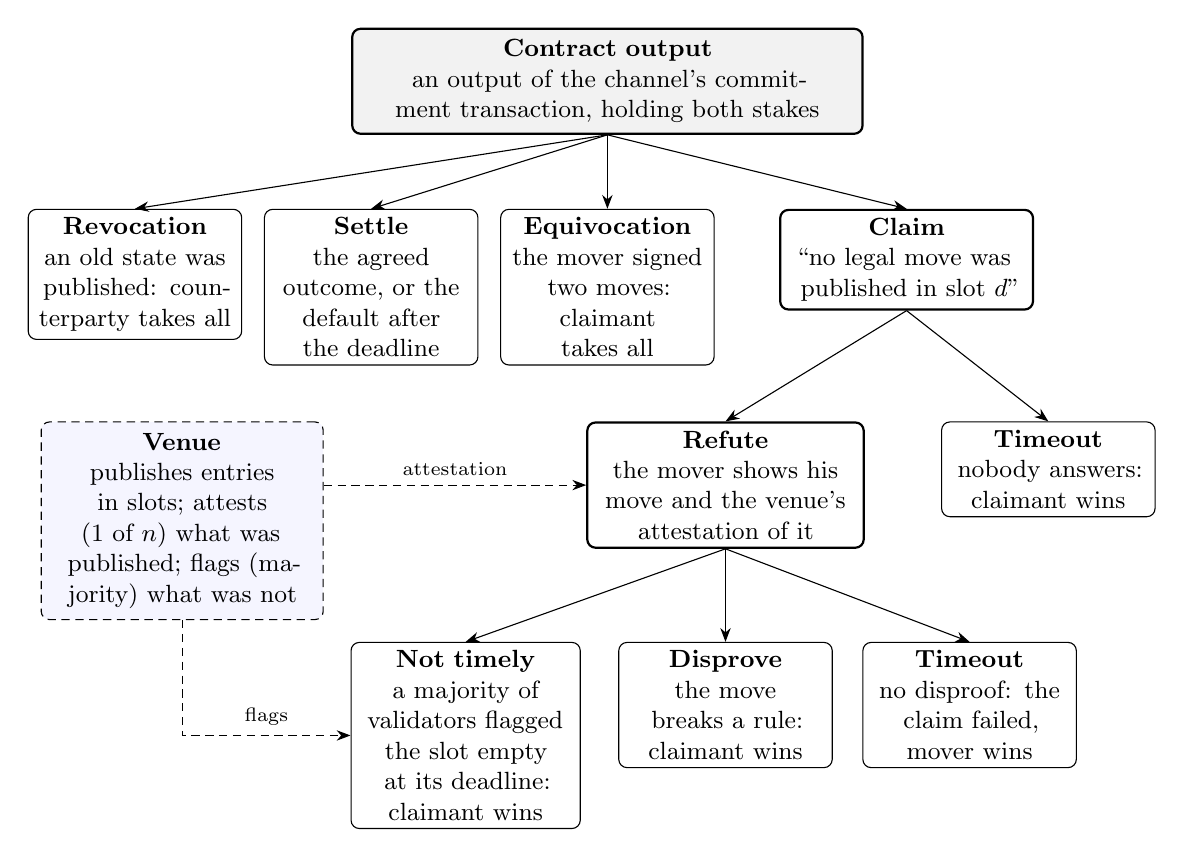
\begin{tikzpicture}[
  font=\small,
  box/.style={draw, rounded corners=3pt, align=center, inner sep=3pt, text width=#1, anchor=north},
  box/.default=25mm,
  cout/.style={draw, thick, fill=black!5, rounded corners=3pt, align=center, inner sep=4pt, anchor=north},
  ven/.style={draw, densely dashed, rounded corners=3pt, align=center, inner sep=4pt, fill=blue!4, anchor=north},
  >={Stealth[length=5pt]},
]
\node[cout, text width=62mm] (C) at (0,0) {\textbf{Contract output}\\ an output of the channel's commitment transaction, holding both stakes};

\node[box] (rev) at (-6,-2.3) {\textbf{Revocation}\\ an old state was published: counterparty takes all};
\node[box] (set) at (-3,-2.3) {\textbf{Settle}\\ the agreed outcome, or the default after the deadline};
\node[box] (eqv) at (0,-2.3) {\textbf{Equivocation}\\ the mover signed two moves: claimant takes all};
\node[box=30mm, thick] (clm) at (3.8,-2.3) {\textbf{Claim}\\ ``no legal move was published in slot $d$''};
\foreach \n in {rev,set,eqv,clm} \draw[->] (C.south) -- (\n.north);

\node[box=33mm, thick] (ref) at (1.5,-5.0) {\textbf{Refute}\\ the mover shows his move and the venue's attestation of it};
\node[box] (to1) at (5.6,-5.0) {\textbf{Timeout}\\ nobody answers: claimant wins};
\draw[->] (clm.south) -- (ref.north);
\draw[->] (clm.south) -- (to1.north);

\node[box=27mm] (nt) at (-1.8,-7.8) {\textbf{Not timely}\\ a majority of validators flagged the slot empty at its deadline: claimant wins};
\node[box] (dis) at (1.5,-7.8) {\textbf{Disprove}\\ the move breaks a rule: claimant wins};
\node[box] (to2) at (4.6,-7.8) {\textbf{Timeout}\\ no disproof: the claim failed, mover wins};
\foreach \n in {nt,dis,to2} \draw[->] (ref.south) -- (\n.north);

\node[ven, text width=33mm] (V) at (-5.4,-5.0) {\textbf{Venue}\\ publishes entries in slots; attests (1 of $n$) what was published; flags (majority) what was not};
\draw[->, densely dashed] (V.east |- ref.west) -- node[above, font=\scriptsize] {attestation} (ref.west);
\draw[->, densely dashed] (V.south) |- node[pos=0.75, above, font=\scriptsize] {flags} (nt.west);
\end{tikzpicture}
\caption{The dispute logic of one contract output, at a high level. Only
the claim and its answers involve the venue: a claim of absence is
answered by the venue's attestation that the move was published, and
that answer is in turn answered either by the game's rules (the move was
illegal) or by the venue again (the move was published too late). Every
branch that pays someone is a Bitcoin transaction prepared in advance;
the arrows are spending conditions, not messages.}
\label{fig:highlevel}
\end{figure}


\subsection{Building a proof of publication ledger}

We can build a single-use seal using Bitcoin itself. That is of course a well known primitive by now, and exemplified in the simple, but useful, OpenTimestamps project LINK. As discussed earlier, it's not practical to use this to adjudicate onchain, because Bitcoin SPV proofs in Script are not practical. If we make a separate proof of publication ledger, we could use proof of work as a consensus mechanism for deciding a canonical chain, or we could use a set of bonded validators, where the security assumption is: if members of the quorum equivocate on the state, their bond can be slashed. This is the equivalent economic security assumption of the reorg threat in the proof of work variant. Let's consider PoW and bonded validator\footnote{We are not calling it proof of stake, because while the consensus algorithm may be similar, it's a notably different security construction than one in which the stake is the tokens of the ledger itself; here the ``stake'' is the bond \emph{in Bitcoin}, a timelocked slashable-to-burn output on the Bitcoin blockchain itself.}.

\subsubsection{Proof of Work}

As already noted, proving inclusion in Bitcoin's PoW chain with its SHA2 linked chain of headers is not practical in Bitcoin Script, without new opcodes (for example CAT for Merkle trees; we defer the details to many other papers and discussions). But since we are designing from scratch, we are not limited to that.

Considering that arithmetic in Bitcoin Script is more or less limited to ``Little Script'' which operates on 4 byte numbers, what we can do is design the proof of work algorithm to use nibble arithmetic only. This is realized in our sample code in n4bitLINK. Note that there had already been a very similar construction made in 2025 by AbdelStark, see stacksat-128LINK. So in general terms, imagine the proof of work hashing uses this nibble based algo, such that proving a hash chain is correct in Bitcoin Script is actually feasible. This would mean a contract participant can post something to the proof of publication ledger, and if their counterparty challenges, saying ``you didn't publish anything'', they can prove that in fact they did, in Script, thus winning the dispute over the pot.

Consider reorgs and canonical history: the key feature of proof of work is that the canonical history is defined by the heaviest chain. So imagine: Alice says ``Bob didn't publish his move'', then Bob says ``yes I did: it's in this PoP ledger block at this height, and here's the header chain back to genesis/checkpoint''. Alice can counter-refute: ``no you didn't: here's an alternate header chain with more weight, proving that yours is not canonical''. This is of course both necessary but also shows the fragility: necessary because otherwise Bob can "mine" a super-cheap chain that costs almost no PoW, fragile because without the kind of enormous weight of something like Bitcoin's PoW chain, reorgs could be easy and frequent even without adversarial behavior.

The least desirable aspect of the PoW option is in there: it's that this costs significant resources to maintain, otherwise it offers no security at all. How are miners compensated for this work? Merge mining seems not to apply straightforwardly, but the biggest count against this idea is the following:

\textbf{There is not a simple transaction fee paying process}, since all contracts are settled in Lightning channels (one can concoct something here, but it's not simple); the contract participants can, by the very nature of proof of work's lottery, never know in advance who the miner will be. If the ledger is not a blockchain with its own coin and own set of consensus rules, there is no viable way to create a positive incentive to include publications.

\subsubsection{Bonded validator quorum}

The alternative is to reach consensus over a quorum, on the blocks of the proof of publication ledger.

It turns out that with careful thought, it's possible to construct a version of this that is both sufficiently efficient to enforce the necessary rules in Script, and also that has the right kind of both positive and negative incentives, purely measured in bitcoin, without inserting a new altcoin.

A naive idea of how to do this hits a snag: Bitcoin Script can read Winternitz signatures in a couple of kilobytes; weighty but OK. It cannot, directly, read Schnorr or BLS signatures on arbitrary messages (the former without CHECKSIGFROMSTACK, the latter .. well that would be a much bigger consensus update!). The latter two can support an aggregated signature; the former (Winternitz, or Lamport) cannot. To assess 66 out of 100 Winternitz signatures in a Bitcoin signature seems patently absurd.

Therefore we consider the natural question: can you reproduce the one-time nature of hash-based OTS schemes in an elliptic curve context? We claim that you can, using something we'll call EC-OTS; the detailed explanation is deferred to LINK. That construction might be of independent interest, since it gives the same basic effect as a hash-based WOTS, but using EC curve points instead.

But taking that construction and saying ``we'll have a $\frac{2}{3}$ threshold attest to state updates in an EC OTS verifiable in Script'' really doesn't give you what you need.

What you need:

\begin{itemize}
\item \textbf{Liveness} : can never be promised, just like in a proof of work chain, but if \emph{any} member of the validator can enter your publication in a slot, then some approximate ``1 of $n$ liveness'' can be claimed, and this is an acceptable security model.
\item \textbf{A large enough quorum}: Credibility of the above as well as what follows, requires some relatively large, heterogeneous and ideally permissionless-entry set of validators. This naturally leads to thinking of FROST-style thresholds, with O(1) publication, but (see next entry) that is not actually viable and so we go with a trick to make thresholds of 50 of 100 be viable. Even figures 10 times higher than that are \emph{theoretically} possible, but in practice we would not go much higher.
\item \textbf{Fraud is attributable}: this is the reason why a naive FROST-style threshold is unworkable: by its nature, such a threshold signature cannot reveal which members of the validator set committed the fraud. And punishing the entire set of such members when only a threshold have committed the fraud, is clearly unworkable. To make fraud attribution feasible we use what we call a ``one-bit signature'':  $t$ of $n$ OP\_CHECKSIGADD operations can prove that a binary true/false was attested to. More on that in a moment.
\item \textbf{Positve incentives in bitcoin}: this is possible in a more general ``sidechain'' model (pay fees to move around coins on the sidechain), but this is not a sidechain, nor any kind of blockchain: the only consensus maintained on the ledger is the canonical history of publications; the semantics of the publications are none of its business. Here we have validators post bonds on bitcoin (timelocked coins) and receive fees for its publication efforts, atomically with those publications, over Lightning channels, using adaptors. This incentivizes honest participation and disincentivizes fraud or dishonesty.
\end{itemize}

You may be wondering why we insist on \emph{attributable} fraud. Without attribution, users of the ledger cannot discern which members they do not want to use in future, if something fraudulent is published. It's also possible, with attribution, to go further, and we do: we have equivocation fraud reveal a secret which can be used to burn the bonded coins (coins locked to a CLTV output), but without covenants, this is not a simple burn, it is more a miner fee-race burn: so the money game-theoretically is more or less guaranteed to end up with the miner of the next block after the secret publication. This is usually, realistically, a substantial punishment for a fraudulent validator; theoretically they can collude with bitcoin miners, but it would have to be a substantial fraction of miners to even have a chance of recouping, so that is largely theoretical.

\subsection{What the proof of publication ledger attests to}

We'll continue to use the two simple motivating examples: tic-tac-toe, and chess. We'll discuss external facts, i.e. something not limited to a 2 player game, in Section LINK.

What would an attestation look like? Probably a variant of:

\[ (S, m, S', t) \]

where we set a notation of $S$ for the game's internal state (e.g. chess: piece positions on the 64 square board plus a couple other details like castling), $m$ for the move being presented, and $t$ an optional extra defining ``terminal'' state: undefined, win A, win B, draw etc. depending, again, on the game.

Specific cases \emph{may} justify condensing this; the most natural one might be removing $S$, the state \emph{before} the player's move.

Each player attests to a move choice, of course; but there's a subtlety that affects the question of how condensed the game state $S$ attested to should be. In the case of tictactoe it can be as few as 20 or so bits; in the case of chess it can be \~ 35 bytes.



The subtlety is that the court sees nothing but what the dispute puts in
front of it. When the claimant disputes a move, the only facts available
in Script are the venue's attestations of two consecutive entries: the
one at the disputed slot and the one before it. So the attested state
must be \emph{self-sufficient}: everything the rules need in order to
judge a move must be recoverable from the pair $(S, S')$ plus the move
itself, with no appeal to the rest of the game's history. For
tic-tac-toe this is trivial (the board and whose turn it is). For chess
it means the state carries castling rights, the en-passant square, the
side to move and a status field, and it rules out adjudicating rules
that need the whole history (threefold repetition) unless a digest of
that history is itself part of the state.

Once the state is self-sufficient, the natural condensation follows: an
entry need carry only $(m, S', t)$, since the previous slot's entry
already carries $S$. The court reads both entries out and judges the
triple $(S, m, S')$. This is the form we use: each entry's \emph{head}
(48 bytes) holds the new state, the move and the status, the region the
mover signs; the entry carries the mover's one-time signature over that
region beside the head; and a dispute reads out the heads at slots $d-1$
and $d$. The mover's signature matters as much as the venue's: a venue
attestation proves an entry was \emph{published}, the mover's one-time
signature proves the mover \emph{made} it, and a refutation needs both,
or anyone could answer a claim with any junk the venue happened to
seal.

What the court needs from the venue is therefore exactly three kinds of
statement per slot, and nothing about the game:
\begin{enumerate}
\item \emph{this} entry was published in slot $d$ (a positive
  attestation, by whichever member sealed the slot);
\item the member who sealed slot $d$ was member $i$ (so that it can be
  paid, and blamed);
\item slot $d$ carried no entry at its deadline (a negative statement,
  by a majority of members).
\end{enumerate}
Section~\ref{sec:venue} describes how the venue produces these, and
Section~\ref{sec:graph} how a Bitcoin script consumes them.

\section{The venue}
\label{sec:venue}

The venue is a set of $n$ bonded members that publish entries in
numbered \emph{slots}. It is not a blockchain in the usual sense: it has
no coin, executes nothing, and maintains no state beyond the record of
what was published in each slot. It is closer to a schedule of one-time
attesters than to a chain.

\subsection{Slots and the clock}

Slot $d$ has a deadline $T_d = t_0 + d\ell$, where $t_0$ is fixed at the
contract's open and $\ell$ is the venue's slot length (seconds to
minutes). Move $d$ of a game must appear in slot $d$. The venue keeps
wall-clock time: members judge ``empty by $T_d$'' against their own
clocks, which need agree only to within ordinary clock skew. Bitcoin's
clock is read in exactly one place, the earliest time an absence claim
for slot $d$ may be broadcast, which is an absolute timelock at
$T_d + m$ against median-time-past, with a margin $m$ covering the lag
of median-time-past and a miner's freedom to skew timestamps. All other
windows in a dispute are relative timelocks, where block granularity
only slows a resolution.\footnote{The proof-of-concept counts slots in
Bitcoin blocks (slot $d$ is sealed at height $b_0 + d$), and the scripts
in Section~\ref{sec:graph} are written that way; replacing the height
$b_0 + d + 1 + g$ by the time $T_d + m$ changes one timelock per leaf
and nothing else.} This is the whole point of having a venue: the
per-move clock runs at the venue's pace, and Bitcoin's clock measures
only the $O(1)$ dispute about it.

\subsection{Publishing: one content key, sealed by any member}

A player publishes by sending its entry to any member. The member
\emph{seals} the slot: it produces a block whose 96-byte header carries
the entry's head, and attests the header with the venue's \emph{content
key}, a Schnorr key $X$ that every member holds. The attestation is an
EC-OTS: for every slot $s$, header chunk $j$ and nibble value $v$, the
venue has published in advance an \emph{anticipation point}
$A_{s,j,v}$, and sealing a header with nibbles $v_0 \ldots v_{191}$
reveals the discrete logs $a_{s,j,v_j}$ of the selected points.
Section~\ref{sec:graph:math} gives the construction. Its property for
our purposes is that a Bitcoin script can check, one \op{CHECKSIG} per
chunk, that the venue attested a particular value at a particular
position, with no signature verification over arbitrary messages.

Because the content key is shared, \emph{any} member can seal \emph{any}
slot; a member that is silent is simply skipped. Inclusion therefore
needs only one honest, live member per slot (``1 of $n$ liveness''). A
shared key cannot say who used it, so each member also holds, per slot,
a \emph{proposer} key $P_{i,s} = p_{i,s}G$ and reveals $p_{i,s}$ in the
block it seals. Every refutation on Bitcoin names the member whose block
it relies on (Section~\ref{sec:graph:claim}).

\subsection{Absence: the flag}

The negative statement is a one-bit signature. Each member holds, per
slot, a \emph{flag} key $F_{i,s} = f_{i,s}G$ and reveals $f_{i,s}$ if
slot $s$ carried no entry at $T_s$. A flag is not an attestation of
content; it is a single point whose secret is revealed or not, so a
script counts flags with \op{CHECKSIGADD} at the cost of one key per
member. A refutation relying on a block that $t$ members flagged as
empty at its deadline is killed by the \texttt{not\_timely} leaf. The
threshold is a bare majority, $t = \lceil (n+1)/2 \rceil$: a flag is
one-sided (false emptiness costs $t$ named flaggers; a late block left
standing costs the proposer plus the silence of $n - t + 1$ honest
members), and the two failure costs balance at the majority.

This is what makes timeliness enforceable against a colluding member. A
member that seals a stalling player's move \emph{after} the deadline
produces a perfectly valid attestation, and without flags a refutation
built on it would defeat an honest absence claim. With flags, the honest
majority's on-time statement ``slot $d$ was empty'' outweighs the late
block, and names its sealer.

\subsection{The registry}

Everything a contract needs from the venue is fixed at open. The
\emph{registry} lists the members, their proposer and flag points for
every slot, and the content tables, each co-signed by every member. A
contract pins the registry by root. Members never see contracts: they
publish points in advance and scalars when they seal or flag, and
whoever disputes uses them.

\subsection{Incentives}

\paragraph{Fees.} A mover pays the member that seals its move,
atomically, with a point-locked payment inside the mover's channel. The
lock point is $T = C_h + P_{i,s}$, the sum of the content points the
mover's head selects and the intended sealer's proposer point; its
discrete log is revealed exactly when member $i$ seals exactly that
head in slot $s$ (Section~\ref{sec:graph:fee}). Publication and payment
are one event, as a preimage and a payment are one event in Lightning.

\paragraph{Bonds.} Each member locks bitcoin in a timelocked output on
Bitcoin for the duration of its membership. The lock is a sacrifice of
time value, not a slashable deposit in the baseline design: a member
caught contradicting itself (two blocks at one slot; a lock completed
without the matching block; a backfill against its own flags) is
ejected, losing its future fee stream while its lock sits out its term.
A venue may additionally attach evidence leaves to the bond, spendable
by anyone holding a proof of equivocation; without covenants such a
spend is a fee race, so the bond ends as miner fee, a burn in effect.

\paragraph{The resulting condition.} An equivocation that needs $t$
members is irrational when
\[
  t \cdot \Bigl(\frac{\mathrm{PV}(F)}{n} + L\Bigr) \;>\; G,
\]
where $\mathrm{PV}(F)$ is the present value of the venue's total fee
stream, $L$ the time value of one member's lock, and $G$ the value the
equivocation can extract. For a fixed threshold fraction $t/n$ the
security budget is a fixed share of the venue's fee revenue, whatever
$n$ is: as with Bitcoin's miners, the number of validators buys
decentralisation and liveness, the revenue buys safety.
Section~\ref{sec:security} takes this up.


\section{Contract outputs and the dispute graph}
\label{sec:graph}

This section gives the transaction-level view of a game contract: what
sits on each commitment transaction, which transactions are pre-signed
when a channel state is agreed, which are built at dispute time by one
party alone, and how the venue's attestations enter the scripts as
public-key constants. We use tic-tac-toe as the worked instance
(a $48$-byte entry head, at most $M=9$ moves) and quote chess where the
numbers differ. Throughout, $\U$ is the user and $\Hb$ the hub; each
holds a payment key $P_\U$, $P_\Hb$, and every 2-of-2 leaf below is
\[
  \push{P_\U}\ \op{CHECKSIG}\ \push{P_\Hb}\ \op{CHECKSIGADD}\ \push{2}\ \op{NUMEQUAL}
\]
(or \op{NUMEQUALVERIFY} when the leaf continues), with the witness
carrying $\sigma_\Hb$ then $\sigma_\U$. Timelocks: $\tsd$ is the
channel's \texttt{to\_self\_delay}, $\dl$ the challenge window and
$\dlp$ the additional delay on prover-favourable paths; $b_0$ is the
Bitcoin height the venue's slot count starts from and $g$ a grace
period, so a depth-$d$ absence claim is admissible from height
$b_0 + d + 1 + g$.

\subsection{Keys and venue data fixed at open}
\label{sec:graph:keys}

The two parties agree the contract at an off-chain draft. Beyond the
channel keys, the draft fixes, per depth $d \in 1..M$ (move $d$ is made
by the \emph{mover} $m(d)$, alternating from $\U$ at $d=1$; the other
party is the \emph{claimant} $c(d)$):
\begin{itemize}
\item $K^{\mathrm{ref}}_d$, the mover's \emph{refute key}: a Winternitz
  one-time key (w = 16, HASH160) over the pair of venue heads
  $h_{d-1}\,\|\,h_d$ ($96$ bytes, $192$ message digits plus $3$ checksum
  digits; $48$ bytes at $d=1$, where the prior state is the constant
  empty board);
\item $K^{\mathrm{st}}_d$, the mover's \emph{state key}: a Winternitz
  key over the signed region of the entry (the $3$ state bytes for
  tic-tac-toe; $42$ bytes for chess). The venue entry the mover
  publishes carries this signature inline, so anyone can check
  authorship of a published move without the mover's cooperation;
\item $K^{\mathrm{code}}_d$ (mover) and $K^{\mathrm{ccode}}_d$
  (claimant): Lamport keys over the $2$-bit outcome code $X \in \{\text{UserWins},
  \text{HubWins}, \text{Draw}\}$.
\end{itemize}
From the venue's registry the draft pins, per slot $s$ (slot $s$ is
where move $d=s$ must appear):
\begin{itemize}
\item the \emph{content table} $A_{s,j,v}$, $j \in 0..191$, $v \in
  0..15$: one anticipation point per header chunk per nibble value, all
  under the venue's shared content key (\S\ref{sec:venue});
\item the $n$ members' \emph{proposer points} $P_{i,s}$ and \emph{flag
  points} $F_{i,s}$, $i \in 1..n$, and the flag threshold
  $t = \lceil (n+1)/2 \rceil$.
\end{itemize}
Only the $96$ head chunks of each table ($j \in 80..175$, the entry head
inside the $96$-byte header) are ever embedded in a script; a refutation
reads the head out, not the whole header.

\subsection{The commitment transaction}
\label{sec:graph:commit}

Each channel state $k$ has two commitment transactions, one per
broadcaster, spending the funding output. Beyond \texttt{to\_local} and
\texttt{to\_remote}, the commitment carries one output per open
\emph{contract}: the game output $C$ of value $V$ (both stakes), and,
while a move's attestation fee is in flight, a \emph{fee lock} output
$L$ (\S\ref{sec:graph:fee}). Every contract output is a taproot output
with an unspendable internal key and a tree of named leaves; on the
broadcaster's version every revocable leaf sits beside the standard
revocation leaf
\begin{lstlisting}[style=script]
revoke:  OP_HASH160 (*\push{h_{\mathrm{rev}}}*) OP_EQUALVERIFY (*\push{P_{\mathrm{cp}}}*) OP_CHECKSIG
\end{lstlisting}
where $h_{\mathrm{rev}}$ is the broadcaster's per-state revocation
hash and $P_{\mathrm{cp}}$ the counterparty's payment key, so a revoked
state is swept in full by the counterparty exactly as in Lightning.
Leaves that pay the broadcaster carry an extra $\push{\tsd}\ \op{CSV}\
\op{DROP}$ so that the revocation window is respected; we omit that
prefix below except where it changes the argument.

The game output's tree is
\begin{align*}
  C:\quad & \texttt{revoke},\ \texttt{settle},\
  \texttt{absent}_d\ (d \in 1..M),\ \texttt{exhibit}_d\ (d \in 5..M),\
  \texttt{equiv}_d\ (d \in 1..M).
\end{align*}
\begin{lstlisting}[style=script]
settle:     (*\push{\mathrm{deadline}}*) OP_CLTV OP_DROP  (*\push{\tsd}*) OP_CSV OP_DROP
            2-of-2
absent_d:   (*\push{b_0+d+1+g}*) OP_CLTV OP_DROP  2-of-2-VERIFY  OP_1
exhibit_d:  (*\push{b_0+d+1+g}*) OP_CLTV OP_DROP  2-of-2-VERIFY  (*proposer fragment*)
            (*two-head readout tied to $K^{\mathrm{ref}}_d$, gated on "terminal"*)
equiv_d:    2-of-2-VERIFY  WOTS-VERIFY((*$K^{\mathrm{st}}_d$*))  (*park digits*)
            WOTS-VERIFY((*$K^{\mathrm{st}}_d$*))  (*restore*)
            (*some digit differs*) OP_VERIFY  OP_1
\end{lstlisting}
\texttt{settle} pays $R(\text{empty board})$ after the contract's
deadline and is the fallback when nobody claims. \texttt{absent}$_d$ is
the claimant's \emph{thin absence claim}: ``the mover published no valid
move at slot $d$''. It asserts nothing about venue content, which is
what keeps it two hundred bytes; the venue enters only if the mover
answers. \texttt{exhibit}$_d$ (tic-tac-toe only; chess needs none,
because a mated side simply has no move to refute with) lets the mover
of a terminal move park the attested pair directly and split by its
result. \texttt{equiv}$_d$ pays the non-mover the whole pot on
exhibiting two distinct valid signatures under $K^{\mathrm{st}}_d$: a
Winternitz signature is forced by its message, so two signatures of
different states are a proof that the mover double-signed at that
depth, and no venue data is needed.

\subsection{The claim output and the refutation}
\label{sec:graph:claim}

\texttt{absent}$_d$ is a pre-signed transaction whose single output
$A_d$ carries the claim tree
\begin{align*}
  A_d:\quad & \texttt{refute},\ \texttt{counter}\ (d \ge 2),\
  \texttt{split}_X\ (X \in \{\text{UW},\text{HW},\text{D}\}).
\end{align*}
\begin{lstlisting}[style=script]
split_X:   (*\push{\dl}*) OP_CSV OP_DROP  2-of-2-VERIFY
           LAMPORT-EXPECT((*$K^{\mathrm{ccode}}_d$*), X)  OP_1
counter:   2-of-2-VERIFY  OP_1
refute:    (*\push{P_{m(d)}}*) OP_CHECKSIGVERIFY
           (*\push{P_{1,d}}*) ... (*\push{P_{n,d}}*) (*\push{n}*) OP_PICK (*\push{n{-}1}*) OP_SWAP OP_SUB OP_PICK
                (*\push{n{+}2}*) OP_ROLL OP_SWAP OP_CHECKSIGVERIFY  (*drop $n{+}1$*)
           WOTS-VERIFY((*$K^{\mathrm{ref}}_d$*))               (*192 digits on the stack*)
           AUTHORSHIP((*$K^{\mathrm{st}}_d$*) over the new head's digits)
           OP_TOALTSTACK (*$\times 192$*)
           READOUT((*$A_{d-1,j,\cdot}$*), (*$j \in 80..175$*))          (*prior head*)
           READOUT((*$A_{d,j,\cdot}$*),   (*$j \in 80..175$*))          (*new head*)
           OP_1
\end{lstlisting}
The claimant's \texttt{split}$_X$ is the timeout: after $\dl$ blocks
with no refutation, the claimant reveals its code key to the outcome it
asserts and both pre-signed signatures pay the corresponding
distribution. The mover's \texttt{refute} is the only leaf that touches
the venue, and it does three things in one script:
\begin{enumerate}
\item it names the proposer: the witness supplies an index $i$ and a
  signature under $P_{i,d}$, made with the scalar $p_{i,d}$ that member
  $i$ revealed in the block it sealed (\S\ref{sec:graph:math});
\item it \emph{parks} the two heads: the WOTS verification of
  $K^{\mathrm{ref}}_d$ leaves the $192$ message digits (the nibbles of
  $h_{d-1}\|h_d$) on the stack, and the tied authorship check proves the
  mover's state key signed the new head's state region, so a
  garbage-signed entry cannot be refuted with;
\item it \emph{reads out} the venue: for each head chunk $j$ the script
  pushes the sixteen points $A_{s,j,0..15}$, selects the one indexed by
  the parked digit, and requires a signature under it. Since the digit
  \emph{is} the parked value, the readout ties ``what the venue attested''
  to ``what the mover re-committed'' by construction, one witness
  element per chunk.
\end{enumerate}
The per-chunk readout fragment, with the parked digit coming off the
altstack, is
\begin{lstlisting}[style=script]
OP_FROMALTSTACK  (*\push{A_{s,j,0}}*) ... (*\push{A_{s,j,15}}*)
OP_16 OP_PICK  OP_15 OP_SWAP OP_SUB  OP_PICK      (*select $A_{s,j,v_j}$*)
OP_18 OP_ROLL  OP_SWAP  OP_CHECKSIGVERIFY   (*possession of its secret*)
OP_2DROP (*$\times 8$*)  OP_DROP
\end{lstlisting}
$16 \times 33$ bytes of constants and $20$ opcodes per chunk; $96$
chunks per head. A wrong digit selects a point whose secret nobody
holds, and the leaf aborts.

\texttt{counter} (from $d \ge 2$) is the mover's own thin claim one
depth back, ``the claimant did not move at $d-1$'': the negation of the
claim's dueness. Its output is the depth-$(d-1)$ claim tree verbatim
(without a counter of its own), so a false counter is refuted by the
claimant's attested, signed head at $d-1$ and judged by the ordinary
family, while a true counter means the claim was never due. One level
closes it.

\subsection{The refuted output}
\label{sec:graph:refuted}

\texttt{refute} is pre-signed too (the mover's payment key gates it),
so its output $P_d$ is pinned to the \emph{refuted tree}
\begin{align*}
  P_d:\quad & \texttt{disprove}_\pi\ (\pi \in \Pi_d),\ \texttt{not\_timely},\
  \texttt{split}_X.
\end{align*}
\begin{lstlisting}[style=script]
disprove_(*$\pi$*):  (*\push{\dl}*) OP_CSV OP_DROP  (*\push{P_{c(d)}}*) OP_CHECKSIGVERIFY
             WOTS-VERIFY((*$K^{\mathrm{ref}}_d$*))  PREDICATE((*$\pi$*) over the 192 digits)  OP_VERIFY
             OP_2DROP (*$\times 96$*)  OP_1
not_timely:  (*\push{\dl}*) OP_CSV OP_DROP  (*\push{P_{c(d)}}*) OP_CHECKSIGVERIFY
             (*\push{F_{1,d}}*) OP_CHECKSIG  (*\push{F_{2,d}}*) OP_CHECKSIGADD  ...
             (*\push{F_{n,d}}*) OP_CHECKSIGADD  (*\push{t}*) OP_GREATERTHANOREQUAL
split_X:     (*\push{\dl+\dlp}*) OP_CSV OP_DROP  2-of-2-VERIFY
             LAMPORT-EXPECT((*$K^{\mathrm{code}}_d$*), X)  WOTS-VERIFY((*$K^{\mathrm{ref}}_d$*))
             RESOLUTION(new head) (*$= X$*)  OP_VERIFY  OP_2DROP (*$\times 96$*)  OP_1
\end{lstlisting}
The \emph{disprove family} $\Pi_d$ is the game's rule set expressed as
predicates over the parked tuple (prior state, move, new state): for
tic-tac-toe \texttt{wrong\_slot}, \texttt{cell\_occupied}$_i$,
\texttt{board\_mismatch}$_i$, \texttt{turn\_not\_flipped},
\texttt{status\_mismatch} and so on (about thirty leaves); for chess the
twelve certificate kinds (a piece moving through an occupied square, a
king left in check, \dots) plus a well-formedness leaf, each taking a
small exhibit (a square, an attacker) from the witness. A disprove is
not pre-signed: the claimant builds it at dispute time, copies the
mover's WOTS reveal from the confirmed refutation's witness, signs with
its own key, and takes the pot. \texttt{not\_timely} is the timeliness
disprove (\S\ref{sec:graph:math}): it counts signatures under the
members' flag points and kills a refutation whose slot $t$ members
flagged as empty at its deadline. The mover's \texttt{split}$_X$ is
\emph{self-checking}: unlike the claim output's timeout split, it must
also re-park the pair and prove in script that $R(\text{parked new
state}) = X$, because a refutation carries no adjudicated outcome for
a Lightning-style code-mismatch leaf to judge. It fires only after
$\dl + \dlp$, so every disprove has had its window.

\begin{figure}[t]
\centering
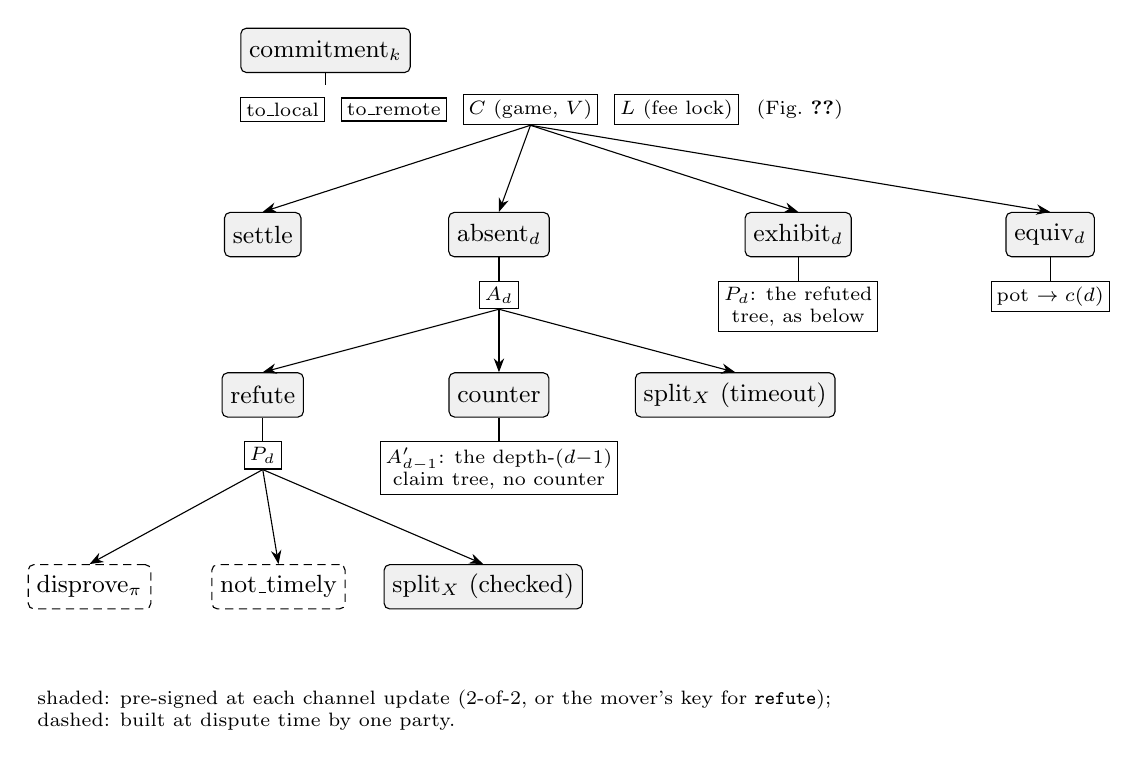
\begin{tikzpicture}[
  font=\small,
  tx/.style={draw, rounded corners=2pt, minimum height=1.6em, inner sep=3pt, align=center},
  pre/.style={tx, fill=black!6},
  run/.style={tx, densely dashed},
  outp/.style={draw, fill=white, inner sep=2pt, font=\scriptsize},
  >={Stealth[length=5pt]},
  every edge/.style={draw, ->},
  node distance=6mm and 9mm,
]
\node[pre] (commit) {commitment$_k$};
\node[outp, below=3mm of commit.south west, anchor=north west] (tl) {to\_local};
\node[outp, right=2mm of tl] (tr) {to\_remote};
\node[outp, right=2mm of tr] (C) {$C$ (game, $V$)};
\node[outp, right=2mm of C] (L) {$L$ (fee lock)};
\draw (commit.south) -- ++(0,-1.5mm);

\node[pre, below=11mm of C, xshift=-34mm] (settle) {settle};
\node[pre, below=11mm of C, xshift=-4mm] (absent) {absent$_d$};
\node[pre, below=11mm of C, xshift=34mm] (exhibit) {exhibit$_d$};
\node[pre, below=11mm of C, xshift=66mm] (equiv) {equiv$_d$};
\foreach \n in {settle,absent,exhibit,equiv} { \draw (C.south) edge (\n.north); }

\node[outp, below=3mm of absent] (Ad) {$A_d$};
\draw (absent) -- (Ad);
\node[pre, below=8mm of Ad, xshift=-30mm] (refute) {refute};
\node[pre, below=8mm of Ad, xshift=0mm] (counter) {counter};
\node[pre, below=8mm of Ad, xshift=30mm] (tsplit) {split$_X$ (timeout)};
\foreach \n in {refute,counter,tsplit} { \draw (Ad.south) edge (\n.north); }

\node[outp, below=3mm of refute] (Pd) {$P_d$};
\draw (refute) -- (Pd);
\node[run, below=12mm of Pd, xshift=-22mm] (disprove) {disprove$_\pi$};
\node[run, below=12mm of Pd, xshift=2mm] (nt) {not\_timely};
\node[pre, below=12mm of Pd, xshift=28mm] (csplit) {split$_X$ (checked)};
\foreach \n in {disprove,nt,csplit} { \draw (Pd.south) edge (\n.north); }

\node[outp, below=3mm of counter, align=center] (Adm) {$A'_{d-1}$: the depth-$(d{-}1)$\\claim tree, no counter};
\draw (counter) -- (Adm);

\node[outp, below=3mm of exhibit, align=center] (Pe) {$P_d$: the refuted\\tree, as below};
\draw (exhibit) -- (Pe);

\node[outp, below=3mm of equiv, font=\scriptsize] (Peq) {pot $\to c(d)$};
\draw (equiv) -- (Peq);

\node[right=1mm of L, font=\scriptsize] {(Fig.~\ref{fig:fee})};

\node[anchor=north west, font=\scriptsize, align=left] at ($(disprove.south west)+(0,-9mm)$)
  {shaded: pre-signed at each channel update (2-of-2, or the mover's key for \texttt{refute});\\
   dashed: built at dispute time by one party.};
\end{tikzpicture}
\caption{The game output $C$ on one commitment and the transactions
hanging off it, per depth $d$. Every output is a taproot tree; the
edges are its leaves. The claim output $A_d$ races the mover's
refutation against the claimant's timeout; the refuted output $P_d$
races the claimant's disproves against the mover's self-checking split;
the counter sends the game one depth back.}
\label{fig:graph}
\end{figure}

\subsection{Pre-signing}
\label{sec:graph:presign}

Every shaded transaction in Figure~\ref{fig:graph} is built and signed
by both parties when a channel state is agreed, on both commitment
versions, and its signatures are exchanged in the same message as the
commitment signature. A script-path sighash commits to the leaf, so
each leaf's transaction needs its own pair of signatures. The counts
are fixed by $M$:
\[
  1 \;+\; M\,(1 + 1 + 3 + 3) \;+\; M \;+\; (M-1)\,(1 + 1 + 3 + 3)
  \;+\; \underbrace{4\,(M-4)}_{\text{tic-tac-toe exhibits}},
\]
that is \texttt{settle}; per depth the claim, its refutation and the
three-plus-three splits; the equivocation exhibit; per depth from $2$
the counter with the previous depth's refutation and splits; and, for
tic-tac-toe, per terminal depth the exhibit with its three splits. With
$M=9$ this is $166$ transactions; for chess with $M=8$ and no exhibit
family, $129$. The disproves and \texttt{not\_timely} are not counted:
they are the challenger's own transactions. Building the graph is
dominated by hashing the refutation scripts (about $100$\,KB each, one
per depth per version); signing $166$ transactions is a few
milliseconds.

\subsection{How the points and signatures connect}
\label{sec:graph:math}

\paragraph{The content attestation.}
The venue's content key is a Schnorr key $X = x G$ shared by its
members. For slot $s$, chunk $j$ and value $v$ the venue derives a
per-statement nonce $r_{s,j,v}$ and publishes the anticipation point
\[
  A_{s,j,v} \;=\; R_{s,j,v} + e_{s,j,v}\,X,
  \qquad R_{s,j,v} = r_{s,j,v}\,G,\quad
  e_{s,j,v} = H(R_{s,j,v},\,X,\,s\,\|\,j\,\|\,v).
\]
Sealing a header $\mathbf{h}$ with nibbles $v_0..v_{191}$ at slot $s$
means revealing, for every $j$, the scalar
\[
  a_{s,j,v_j} \;=\; r_{s,j,v_j} + e_{s,j,v_j}\,x,
  \qquad a_{s,j,v_j}\,G = A_{s,j,v_j},
\]
that is, a Schnorr signature on the statement ``chunk $j$ of slot $s$
is $v_j$'' whose value is its own verification key. Scripts never
verify these signatures; they verify possession of them. The mover
proving that the venue attested $h_d$ signs the refutation transaction
itself with each revealed $a_{d,j,v_j}$ as a private key, and the
readout's \op{CHECKSIGVERIFY} under $A_{d,j,v_j}$ succeeds exactly when
the venue revealed that scalar. Revealing two values at one $(s,j)$ is
the venue equivocating; it is detectable by anyone holding both blocks
and is the object the flags and the proposer bit attribute.

\paragraph{The proposer bit and the flag.}
Content is a $96$-nibble message and costs a table; a statement with no
content costs one point. Each member $i$ therefore holds two one-bit
keys per slot, $P_{i,s} = p_{i,s} G$ (``I sealed slot $s$'') and
$F_{i,s} = f_{i,s} G$ (``slot $s$ carried no entry at its deadline''),
and reveals the scalar when the statement holds: $p_{i,s}$ in the block
it seals, $f_{i,s}$ as data. A revealed scalar is again a private key,
so the disputing party signs its \emph{own} transaction with it. In
\texttt{refute} the proposer fragment selects $P_{i,d}$ by a witness
index and demands a signature under it, so every refutation names the
member that sealed the slot. In \texttt{not\_timely} the claimant
signs under any $t$ of the $F_{i,d}$ and leaves the rest of the
witness slots empty; \op{CHECKSIGADD} counts, an empty signature adds
zero, and the leaf passes iff at least $t$ members flagged. Members
never see the contract or the transaction: they publish scalars, and
whoever disputes uses them. The threshold is a majority because the
flag is one-sided: false emptiness costs $t$ named flaggers, while a
late attestation left standing costs the proposer plus $n-t+1$
silent members, and the two balance at $t = \lceil (n+1)/2 \rceil$.

\paragraph{The parked tuple.}
The refute key is the bridge between the two halves of the script. A
Winternitz signature under $K^{\mathrm{ref}}_d$ on the message
$h_{d-1}\|h_d$ reveals, for message digit $i$ with value $d_i$, the
chain element $\sigma_i = \mathrm{HASH160}^{(d_i)}(\mathrm{sk}_i)$, and
the script checks $\mathrm{HASH160}^{(15-d_i)}(\sigma_i) =
\mathrm{pk}_i$ digit by digit, with the usual checksum digits
preventing a downward forgery. What remains on the stack afterwards is
the $192$ digits themselves. The readout consumes them as the selectors
$v_j$; the disprove predicates and the resolution check read them as
the tuple. Since the key is one-time and the claim, exhibit and counter
contexts are mutually exclusive spends of $C$, the mover can park at
most one tuple per depth, and a disprove built from the confirmed
refutation's witness always judges the tuple the venue attested.

\paragraph{The fee lock.}
A mover pays the member that seals its move, atomically, with a
point-locked payment in the channel (\S\ref{sec:graph:fee}). Let
$C_h = \sum_{j \in \text{head}} A_{s,j,v_j}$ be the sum of the points
the head $h$ selects and $c_h = \sum_j a_{s,j,v_j}$ its discrete log,
which exists exactly when $h$ is attested at $s$. Because the content
key is shared, $c_h$ alone does not say who sealed; the lock's adaptor
point adds the intended proposer's bit:
\[
  T \;=\; C_h + P_{i,s}, \qquad t \;=\; c_h + p_{i,s}, \qquad tG = T.
\]
The payer pre-signs the claim transaction for the payee with a BIP340
adaptor pre-signature: for message $m$ (the claim's sighash), nonce
$k$ with $R' = kG$ and challenge
$e = H(R'+T,\,P_{\text{payer}},\,m)$,
\[
  s' = k + e\,d_{\text{payer}}, \qquad
  \text{verifiable as } s'G = R' + e\,P_{\text{payer}}\ \text{given } T.
\]
Only member $i$ can complete it, $s = s' + t$, which is a valid
signature under nonce point $R'+T$; and once the completed signature is
public the payer extracts $t = s - s'$. The channel machinery sees only
an ordinary point and an ordinary signature.

\subsection{The fee lock output}
\label{sec:graph:fee}

The fee lock $L$ is a second, small contract output on the commitment
while a move's fee is in flight, with the shape of an HTLC:
\begin{lstlisting}[style=script]
revoke:   as above
claim:    [(*\push{\tsd}*) OP_CSV OP_DROP]  2-of-2   (*the payer's half: adaptor under $T$*)
timeout:  (*\push{\mathrm{expiry}}*) OP_CLTV OP_DROP  [(*\push{\tsd}*) OP_CSV OP_DROP]
          (*\push{P_{\text{payer}}}*) OP_CHECKSIG
\end{lstlisting}
\texttt{claim} is pre-signed to the payee's address, the payee's half a
full signature and the payer's the pre-signature above; it is
broadcastable only once completed with $t$. \texttt{timeout} refunds
the payer after \texttt{expiry}. Cooperatively nothing reaches the
chain: the payee, holding $t$, hands it to the payer and proposes the
next channel state with $L$ removed and its value credited, and the
payer's policy accepts iff $tG = T$. A claim with no matching block on
the venue (sealed by nobody, by someone else, or with another head) is
a self-contradiction of member $i$ against the venue's own record, and
is answered by ejection rather than by script.

\begin{figure}[t]
\centering
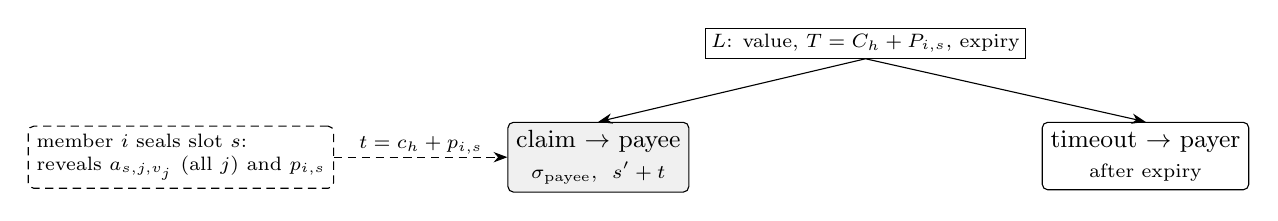
\begin{tikzpicture}[
  font=\small,
  tx/.style={draw, rounded corners=2pt, minimum height=1.6em, inner sep=3pt, align=center},
  outp/.style={draw, fill=white, inner sep=2pt, font=\scriptsize},
  >={Stealth[length=5pt]},
  node distance=5mm and 8mm,
]
\node[outp] (L) {$L$: value, $T = C_h + P_{i,s}$, expiry};
\node[tx, below left=8mm and 2mm of L, fill=black!6] (claim) {claim $\to$ payee\\{\scriptsize $\sigma_{\text{payee}}$, $\ s' + t$}};
\node[tx, below right=8mm and 2mm of L] (to) {timeout $\to$ payer\\{\scriptsize after expiry}};
\draw[->] (L.south) -- (claim.north);
\draw[->] (L.south) -- (to.north);
\node[tx, densely dashed, left=22mm of claim, align=left, font=\scriptsize] (venue) {member $i$ seals slot $s$:\\reveals $a_{s,j,v_j}$ (all $j$) and $p_{i,s}$};
\draw[->, densely dashed] (venue.east) -- node[above, font=\scriptsize, fill=white, inner sep=1pt] {$t = c_h + p_{i,s}$} (claim.west);
\end{tikzpicture}
\caption{The fee lock output. The venue's attestation of exactly the
payer's head at slot $s$ by member $i$ reveals the scalar that completes
the payer's pre-signature; nothing else does.}
\label{fig:fee}
\end{figure}

\subsection{Measured sizes}
\label{sec:graph:sizes}

Table~\ref{tab:sizes} gives virtual sizes as confirmed on a regtest
node with real timelocks, for a five-member venue ($n=5$, $t=3$).

\begin{table}[t]
\centering
\small
\begin{tabular}{llr}
\toprule
transaction & who & vB \\
\midrule
commitment (two balances, one contract) & broadcaster & $\approx 240$ \\
\texttt{absent}$_d$ & claimant & $188$ \\
\texttt{split}$_X$ (timeout, off $A_d$) & claimant & $193$--$201$ \\
\texttt{counter} & mover & $178$ \\
\texttt{refute}, tic-tac-toe, $d \ge 2$ & mover & $\approx 34{,}800$ \\
\texttt{refute}, chess, $d \ge 2$ & mover & $36{,}607$ \\
\texttt{refute}, chess, $d = 1$ (one head) & mover & $19{,}532$ \\
\texttt{disprove}, chess (one exhibit) & claimant & $\approx 4{,}950$ \\
\texttt{not\_timely} ($3$ of $5$ flags) & claimant & $254$ \\
\texttt{split}$_X$ (checked, off $P_d$) & mover & $\approx 4{,}900$ \\
fee \texttt{claim} & payee & $171$ \\
fee \texttt{timeout} & payer & $147$ \\
\bottomrule
\end{tabular}
\caption{Confirmed virtual sizes. A stall costs the claimant two small
transactions at any depth; the refutation is the one large transaction
and is paid by the party that answers a claim, its cost being the
venue readout ($96$ possession proofs per head, $16$ points each, as
script constants) rather than any signature or hash chain.}
\label{tab:sizes}
\end{table}

The shape of the costs is the point of the design. A stall, the common
case, is an absence claim and a timeout: under $400$ vB whatever the
depth of the game. The venue is read out on Bitcoin only when a party
answers a claim, and then once, in a transaction whose size is fixed by
the header format and not by the game; the game's own rules cost a few
kilobytes per disprove, and a chess rule and a tic-tac-toe rule are
the same shape of leaf. Every per-member statement of the venue is one
point in a script and one signature in a witness, so the number of
members changes the graph by tens of bytes per leaf.


\section{A game from open to close}
\label{sec:lifecycle}

Putting the pieces together for one game, and following the branches of
Figure~\ref{fig:highlevel}:

\begin{description}[style=nextline]
\item[Open.] The players agree the contract in their channel: stakes,
  depth limit $M$, the registry root, and the one-time keys per depth.
  They sign the new commitment and the graph of Section~\ref{sec:graph}.
\item[Honest play.] Each move is an entry published on the venue in its
  slot, with its fee paid through the fee lock, and an ordinary channel
  update between the players. At the end, the loser folds: the channel
  is updated to the result and the contract output disappears. Nothing
  reaches Bitcoin.
\item[A stall.] The mover publishes nothing in slot $d$. After $T_d+m$
  the claimant broadcasts the absence claim, then after $\delta$ the
  timeout split. Two small transactions, under $400$ vB, at any depth.
\item[A false stall claim.] The mover did publish. He answers with the
  refutation: the venue's attestation of his entry and the previous
  one, his own signature, and the name of the sealing member. The
  claimant has nothing to disprove; after $\delta + \delta'$ the mover's
  checked split pays him.
\item[An illegal move.] The mover published and signed an illegal move,
  and answers a claim with it. The claimant copies the mover's
  re-commitment from the confirmed refutation's witness and spends the
  one disprove leaf the move violates.
\item[A late move.] A member colluding with the mover sealed his move
  after $T_d$. The honest majority flagged slot $d$ as empty at $T_d$;
  the claimant spends \texttt{not\_timely} with $t$ flags.
\item[Equivocation by a player.] The mover signed two different moves at
  depth $d$ (for instance, one to the venue and another to the
  counterparty). Two signatures under a one-time key at one depth are
  their own proof; the \texttt{equiv} leaf pays the claimant, with no
  venue data.
\item[A revoked state.] As in Lightning.
\end{description}

The asymmetry of cost is deliberate. The common failure, a stall, is
cheap to prove. The expensive transaction, the refutation, is paid by
the party answering a claim, and a party answers only when it will win.

\section{Beyond games: a public clock and a seal}
\label{sec:beyond}

\subsection{Two different services}

The argument so far rested on one impossibility: between two parties,
whether a message was delivered cannot be decided by anyone else. The
receiver can always deny receipt, the sender can always claim to have
sent, and there is no evidence of non-receipt; this is the fair-exchange
impossibility without a trusted third party~\cite{pagnia}. A contract
therefore cannot punish silence unless messages go somewhere the judge
can see. That somewhere must provide two things together: a record of
what was made available (publication), and deadlines against which
the record is read (a clock). We call the combination a \emph{public
clock}. Bitcoin is one, at the cost of a transaction per message; the
venue is one off-chain.

A single Bitcoin block provides three things at once: a clock, a
publication, and uniqueness (one chain, one spend per output). Because
they arrive together they are easily conflated. Off-chain they separate:
\begin{itemize}
\item \textbf{A public clock} is what a two-party game needs. The
  venue's per-slot record must be \emph{decided} (the flag majority), but
  no reader other than the two players ever consults it, so nothing is
  gained by one player being shown a different record than the other: the
  players' own one-time keys already forbid them from signing two
  versions of a move.
\item \textbf{A seal} is what a \emph{shared fact} needs: a fact that
  many contracts read, such as the owner of a name or the set of bids in
  an auction. If the venue could show one record to one contract and a
  different record to another, each would settle on a different world.
\end{itemize}

\subsection{Shared facts, and what defends them}

A true single-use seal (a Bitcoin output) reaches a contract only
through a spend in the contract's own inputs; that is how Lightning's
funding output works. A fact carried as \emph{data}, whether a venue
attestation, a Merkle root or a Bitcoin \texttt{OP\_RETURN}, can only
be exhibited to a script, and a script cannot tell which of two
conflicting exhibits is canonical without verifying the chain it came
from, which is impractical. A seal on Bitcoin (anchoring the venue's
record in a single-use output chain) therefore gives uniqueness to
\emph{clients} running nodes, but not to contracts.

For contracts, uniqueness of a shared fact is economic: two attestations
at one slot are an unambiguous, attributable equivocation by the venue,
whichever of them was anchored, and the condition of
Section~\ref{sec:venue} must hold with $G$ the value extractable from
\emph{all} contracts relying on the slot. For a two-party game $G$ is one
pot. For a shared fact it is an aggregate, measured against the
franchise of the members who equivocate. We take this as the limitation
of the system for shared facts: they are secure up to a value set by the
venue's fee revenue, bounded, and best suited to facts whose total
reliance is bounded and known when they are published. An auction is
such a fact; a long-lived registry is not.

\section{Storage contracts: Filecoin without an altcoin}
\label{sec:storage}

We return to the example of the introduction.

\paragraph{Set-up.} The customer erasure-codes and encrypts its data,
splits it into chunks of a few hundred bytes, and computes a Merkle root
$R$ over them. A contract in the customer's channel with the provider
fixes $R$, the number of chunks, an epoch length, a fee per epoch and
the provider's bond $B$. The data is handed over off-chain.

\paragraph{Each epoch is two moves.} The customer publishes a challenge,
an index $i$, on the venue. The provider must publish chunk $c_i$ with
its Merkle path to $R$ in the next slot. The fee for the epoch is paid in
the channel as usual; the bond stays locked.

\paragraph{Disputes are the game's disputes.} A missing response is an
absence claim, refuted only by a venue attestation of a timely response.
A wrong response is a disprove leaf that checks a Merkle path (SHA-256,
native in Script; the chunk must fit a 520-byte stack element). A false
claim by the customer is answered by the attested response. The
contract graph is the chess graph with a different disprove family: the
``move'' is a challenge or a response, and the ``rule'' is a path check.

\paragraph{What it proves.} A provider that has discarded a fraction
$f$ of the chunks survives each uniformly chosen challenge with
probability $1-f$. Because the data was erasure-coded, the customer
needs only a sufficient fraction, so a provider passing most challenges
holds a recoverable copy: this is a proof of retrievability in the sense
of Juels--Kaliski and Shacham--Waters~\cite{jk,sw}. It proves
retrievability, not that the provider itself stores the data; for the
customer that is usually what matters. Responses are public on the
venue, hence the encryption. The contract's depth limit bounds its
term; longer terms are renewed by cooperative refresh, and the default
at the horizon must favour the customer.

\paragraph{What is new.} Paying for proofs of retrievability over
Bitcoin has been proposed before: contingent service payments on
Bitcoin for exactly this~\cite{zkcsp}, recurring variants~\cite{rcpor},
periodic challenge-and-pay over a payment channel~\cite{scrypt}, and
per-download payments with a bond and fraud proof over
Lightning~\cite{bitstream}. All are \emph{pay on success}: if the
provider does not answer, the customer does not pay, and the only
penalty for losing the data is lost future income. No two-party
construction can do better, because silence cannot be adjudicated
between two parties. With a public clock ``no timely response in epoch
$k$'' is a fact, so the provider's \emph{bond} is forfeited for absence,
not merely its payment withheld, and the whole schedule runs off-chain.

\section{A sealed-bid auction}
\label{sec:auction}

An auction is the simplest useful contract that is not two-party. A
seller auctions a lot; each bidder, and the seller, has a channel with a
hub $\Hb$; every party's contract is a two-party contract with $\Hb$,
and all of them settle on one shared fact: the set of bids published on
time.

\paragraph{Phases.} Bidders publish commitments
$H(\mathit{bid}\,\|\,\mathit{salt}\,\|\,\mathit{key})$ by a commit slot
$s_c$ and reveal them by a reveal slot $s_r$. A bidder locks
$L_i \ge \mathit{bid}_i$ in its contract, over-locking by a random amount
so that $\Hb$ learns nothing before the reveals. An unrevealed
commitment forfeits a deposit $\pi$. Venue slots carry a \emph{set} of
entries for this: the attested head is a Merkle root, and an entry is
exhibited by its path.

\paragraph{The outcome is a pointer claim.} Settlement is claimed as
``winner $w$ at price $p$, where $p$ is bid $k$'', not computed. The
claim is refuted by exhibiting a timely revealed bid above $w$'s, a
timely revealed bid other than $w$'s above $p$, or by showing that bid
$k$ is not a timely reveal. Each refutation is one inclusion path and
one comparison; the number of bidders never enters a leaf. Completeness
comes from the same leaves: an omitted bid is exhibited with its
timeliness, and the seller's contract can exhibit \emph{any} omitted
bid, so $\Hb$ cannot suppress the high bid in favour of a shill.

\paragraph{The legs.} As with a routed payment, the hub's contracts net
to zero: in the seller's contract the lot goes to $\Hb$ against $p$, and
in the winner's the lot goes to the winner against $p$; losers are
refunded. The legs are atomic because they settle on the same fact.

\paragraph{Delivering the lot.} If the lot is a Bitcoin-native asset
(RGB or Taproot Assets), it is a Bitcoin output: the seller commits it
into the contract output at open and delivery is a branch of the
pre-signed graph, so the seller cannot withhold it later. Each graph
transaction the asset passes through carries its asset transition,
built in advance using outputs of the same transaction as seals; the
asset's history is published on the venue at set-up so the winner can
validate it. If the lot lives on another chain, the auction sells the
right to be the counterparty of an atomic swap at price $p$, and the
seller's option to walk away can only be priced, by a deposit forfeited
on timeout.

\paragraph{Its security.} The bid set is a shared fact. An equivocating
venue could show the seller's contract a high price and the winner's a
low one, at the hub's expense. That is the limitation of
Section~\ref{sec:beyond}, and here it is benign: the value at stake is
bounded by the auction and known when its slots are published, so the
fee for the closing slot can be sized to it.

\paragraph{What is still to build.} Set-valued slots, the pointer-claim
graph, and settlement at a variable price (either a grid of pre-signed
splits, one per price bucket, or payouts decomposed into binary-weighted
outputs).

\section{Security}
\label{sec:security}

Table~\ref{tab:security} lists what can go wrong and what prevents it.
The assumptions fall into five classes:
\begin{itemize}
\item \textbf{Cryptographic}: holds unconditionally given the primitives
  (one-time signatures, Schnorr, SHA-256) and Script.
\item \textbf{Lightning's}: a party watches the chain and responds within
  its windows; fees for pre-signed transactions can be bumped.
\item \textbf{1 of $n$}: at least one member is honest and live during
  the relevant slot.
\item \textbf{Majority}: fewer than $t$ members collude.
\item \textbf{Economic}: misbehaviour is attributable and costs more than
  it gains; bounded by the condition of Section~\ref{sec:venue}.
\end{itemize}

\begin{table}[H]
\centering
\small
\begin{tabular}{>{\raggedright\arraybackslash}p{44mm}>{\raggedright\arraybackslash}p{62mm}>{\raggedright\arraybackslash}p{30mm}}
\toprule
threat & defended by & assumption \\
\midrule
publishing a revoked channel state & revocation leaf & Lightning's \\
an illegal move & disprove family, from the refutation's witness & cryptographic \\
answering a claim with an entry the mover did not sign & authorship check in \texttt{refute} & cryptographic \\
a player signing two moves at one depth & \texttt{equiv} leaf & cryptographic \\
a stall & absence claim and timeout & Lightning's \\
a false absence claim & refutation with the venue's attestation & 1 of $n$ (some member sealed the move) \\
censorship of a mover (no member seals) & nothing in Script; fee income, member independence & 1 of $n$ \\
a late seal colluding with the mover & \texttt{not\_timely}: $t$ flags & majority \\
false flags against a timely move & none in Script; flaggers named, ejected & majority; economic \\
two blocks at one slot & proposer named; ejection; optional burn & economic ($G$: one pot) \\
fee lock completed without sealing & self-contradiction against the venue's record; ejection & economic \\
the venue halting & none: see below & --- \\
a shared fact shown differently to different contracts & attribution; ejection; optional burn & economic ($G$: aggregate) \\
refusing to refresh at the horizon & the horizon's default outcome & design \\
\bottomrule
\end{tabular}
\caption{Threats and their defences.}
\label{tab:security}
\end{table}

\paragraph{Where the cryptography ends.} Everything about a game's
\emph{content} is cryptographic: a move is legal or a disprove leaf
fires, a player signs once per depth or loses, a revoked state is swept.
Everything about \emph{time} rests on the venue: that a move was
published is a 1-of-$n$ fact, that it was published \emph{on time} is a
majority fact. This split is the design's central trade. Content is
expensive to adjudicate and made cheap by the disprove family; time is
impossible to adjudicate between two parties and made possible by the
venue.

\paragraph{Censorship.} A mover whose entry no member will seal loses by
absence. This is theft-shaped, not merely a delay, and nothing in Script
prevents it. It requires every member to refuse for the whole slot, and
so is defended by the independence of the members (operators,
jurisdictions, hosts) and by the fees each forgoes; bonds, which punish
only self-contradiction, do not reach it. A forced-inclusion path
through Bitcoin (an \texttt{OP\_RETURN} the venue must honour) is a
possible backstop.

\paragraph{The majority.} Flags are the only place the design needs a
threshold, and it is there for \emph{order}, not for stake: two blocks
by two members (``slot $d$ is empty'', ``slot $d$ holds this move'')
cannot be ordered by any third fact, so canonical timing needs agreement
among the members, or an external clock. A colluding majority can kill
an honest mover's refutation with false flags; the flags are signatures,
so the colluders are named, and the residual falls on a party who knows
whom to pursue.

\paragraph{Venue failure.} If the venue stops altogether, nothing can
be published, and an absence claim against whoever is on move succeeds.
In the present design a dead venue therefore decides games against the
player on move. Requiring the claimant to show the flags (the positive
statement ``slot $d$ was empty'') \emph{in the claim itself} would turn
this into a liveness failure (no flags, no claim; the contract settles by
its default at the deadline), at the price of letting a colluding
majority protect a staller by withholding flags. The choice is between
the two residuals, and it is open.

\paragraph{Economic security, and its limit.} The bond and the fees
defend what is attributable. For two-party contracts the gain from any
venue misbehaviour is at most one pot, and a venue whose members' fee
franchise exceeds the largest pot in flight has no reason to misbehave.
For shared facts the gain is the sum over all contracts relying on a
slot, and the same franchise must cover it. We state this as the
limitation of the system rather than engineer around it: the only ways
to remove it are verifying the venue's chain in Script (SPV, impractical)
or turning the fact into Bitcoin outputs that each contract spends,
which works only for facts of a few bits fixed in structure long in
advance.

\section{Related work}
\label{sec:related}

ForceMove~\cite{forcemove} and state channels are the paradigm we
modify; Lightning~\cite{lightning} the base we build on. Single-use seals
and proof of publication are due to Todd~\cite{toddseals}, and
OpenTimestamps~\cite{ots} is their simplest deployment; RGB~\cite{rgb}
builds client-side-validated assets on them, and its companion Prime
design places commitments in a dedicated header chain anchored to
Bitcoin. The bonded, Bitcoin-collateralised validator set with one-time
signatures is Linus's Coins and Stakechains~\cite{coins}; what is new
here is that the venue settles no value and carries no asset, and that
its attestations are read in Bitcoin Script. BitVM~\cite{bitvm} settles
arbitrary computation on Bitcoin by bisection; we avoid on-chain
bisection by giving each game a family of single-step disprove leaves.
StackSat-128~\cite{stacksat} is a Script-friendly hash designed for the
proof-of-work alternative. For storage, see
Section~\ref{sec:storage}.

\section{Conclusion}

Lightning cannot adjudicate silence, and that single gap is what keeps
games, service agreements and auctions off it. A venue that publishes
in slots, attests what it published with signatures a Bitcoin script can
read, and flags by majority what it did not, closes the gap with
$O(1)$ transactions per dispute and no change to Bitcoin. Content stays
cryptographic; time becomes a 1-of-$n$ and majority fact about a bonded,
fee-paid set of members; shared facts are secured economically, up to a
bound set by the venue's revenue.


\begin{thebibliography}{99}

\bibitem{lightning} J.~Poon and T.~Dryja. The Bitcoin Lightning Network: Scalable off-chain instant payments, 2016. \url{https://lightning.network/lightning-network-paper.pdf}

\bibitem{forcemove} T.~Close and A.~Stewart. ForceMove: an $n$-party state channel protocol. Magmo, 2018.

\bibitem{pagnia} H.~Pagnia and F.~C.~G\"artner. On the impossibility of fair exchange without a trusted third party. Technical report TUD-BS-1999-02, Darmstadt University of Technology, 1999.

\bibitem{toddseals} P.~Todd. Preventing consensus fraud with commitments and single-use-seals, 2016. \url{https://petertodd.org/2016/commitments-and-single-use-seals}

\bibitem{ots} OpenTimestamps. \url{https://opentimestamps.org}

\bibitem{rgb} RGB Protocol. \url{https://rgb.info}

\bibitem{coins} R.~Linus. Coins: a billion Bitcoin users, 2020; R.~Linus and B.~Tse, Stakechains, CoDecFin 2022.

\bibitem{bitvm} R.~Linus. BitVM: compute anything on Bitcoin, 2023.

\bibitem{stacksat} AbdelStark. StackSat-128, 2025.

\bibitem{jk} A.~Juels and B.~S.~Kaliski. PORs: proofs of retrievability for large files. ACM CCS 2007.

\bibitem{sw} H.~Shacham and B.~Waters. Compact proofs of retrievability. ASIACRYPT 2008.

\bibitem{zkcsp} M.~Campanelli, R.~Gennaro, S.~Goldfeder and L.~Nizzardo. Zero-knowledge contingent payments revisited: attacks and payments for services. ACM CCS 2017. \url{https://eprint.iacr.org/2017/566}

\bibitem{rcpor} A.~Abadi, S.~J.~Murdoch and T.~Zacharias. Recurring contingent payment for proofs of retrievability, 2021. \url{https://eprint.iacr.org/2021/1145}

\bibitem{scrypt} sCrypt. Pay for storage using proof of retrievability on Bitcoin. \url{https://scryptplatform.medium.com/pay-for-storage-using-proof-of-retrievability-on-bitcoin-d5f2df009e1}

\bibitem{bitstream} R.~Linus. BitStream: decentralized file hosting incentivised via Bitcoin payments, 2023. \url{https://robinlinus.com/bitstream.pdf}

\end{thebibliography}

\end{document}
